% This is "sig-alternate.tex" V1.9 April 2009
% This file should be compiled with V2.4 of "sig-alternate.cls" April 2009
%
% This example file demonstrates the use of the 'sig-alternate.cls'
% V2.4 LaTeX2e document class file. It is for those submitting
% articles to ACM Conference Proceedings WHO DO NOT WISH TO
% STRICTLY ADHERE TO THE SIGS (PUBS-BOARD-ENDORSED) STYLE.
% The 'sig-alternate.cls' file will produce a similar-looking,
% albeit, 'tighter' paper resulting in, invariably, fewer pages.
%
% ----------------------------------------------------------------------------------------------------------------
% This .tex file (and associated .cls V2.4) produces:
%       1) The Permission Statement
%       2) The Conference (location) Info information
%       3) The Copyright Line with ACM data
%       4) NO page numbers
%
% as against the acm_proc_article-sp.cls file which
% DOES NOT produce 1) thru' 3) above.
%
% Using 'sig-alternate.cls' you have control, however, from within
% the source .tex file, over both the CopyrightYear
% (defaulted to 200X) and the ACM Copyright Data
% (defaulted to X-XXXXX-XX-X/XX/XX).
% e.g.
% \CopyrightYear{2007} will cause 2007 to appear in the copyright line.
% \crdata{0-12345-67-8/90/12} will cause 0-12345-67-8/90/12 to appear in the copyright line.
%
% ---------------------------------------------------------------------------------------------------------------
% This .tex source is an example which *does* use
% the .bib file (from which the .bbl file % is produced).
% REMEMBER HOWEVER: After having produced the .bbl file,
% and prior to final submission, you *NEED* to 'insert'
% your .bbl file into your source .tex file so as to provide
% ONE 'self-contained' source file.
%
% ================= IF YOU HAVE QUESTIONS =======================
% Questions regarding the SIGS styles, SIGS policies and
% procedures, Conferences etc. should be sent to
% Adrienne Griscti (griscti@acm.org)
%
% Technical questions _only_ to
% Gerald Murray (murray@hq.acm.org)
% ===============================================================
%
% For tracking purposes - this is V1.9 - April 2009

\documentclass{sig-alternate}

\begin{document}

\newcommand{\comments}[1]{}
\newcommand{\Enso}{Ens\={o}}

%
% --- Author Metadata here ---
\conferenceinfo{WOODSTOCK}{'97 El Paso, Texas USA}
%\CopyrightYear{2007} % Allows default copyright year (20XX) to be over-ridden - IF NEED BE.
%\crdata{0-12345-67-8/90/01}  % Allows default copyright data (0-89791-88-6/97/05) to be over-ridden - IF NEED BE.
% --- End of Author Metadata ---

\title{\Enso: Extensible interpreters for DSL workbenches}
%
% You need the command \numberofauthors to handle the 'placement
% and alignment' of the authors beneath the title.
%
% For aesthetic reasons, we recommend 'three authors at a time'
% i.e. three 'name/affiliation blocks' be placed beneath the title.
%
% NOTE: You are NOT restricted in how many 'rows' of
% "name/affiliations" may appear. We just ask that you restrict
% the number of 'columns' to three.
%
% Because of the available 'opening page real-estate'
% we ask you to refrain from putting more than six authors
% (two rows with three columns) beneath the article title.
% More than six makes the first-page appear very cluttered indeed.
%
% Use the \alignauthor commands to handle the names
% and affiliations for an 'aesthetic maximum' of six authors.
% Add names, affiliations, addresses for
% the seventh etc. author(s) as the argument for the
% \additionalauthors command.
% These 'additional authors' will be output/set for you
% without further effort on your part as the last section in
% the body of your article BEFORE References or any Appendices.

\numberofauthors{3} %  in this sample file, there are a *total*
% of EIGHT authors. SIX appear on the 'first-page' (for formatting
% reasons) and the remaining two appear in the \additionalauthors section.
%
\author{
% You can go ahead and credit any number of authors here,
% e.g. one 'row of three' or two rows (consisting of one row of three
% and a second row of one, two or three).
%
% The command \alignauthor (no curly braces needed) should
% precede each author name, affiliation/snail-mail address and
% e-mail address. Additionally, tag each line of
% affiliation/address with \affaddr, and tag the
% e-mail address with \email.
%
% 1st. author
\alignauthor
Ben Trovato\\
       \affaddr{Institute for Clarity in Documentation}\\
       \affaddr{1932 Wallamaloo Lane}\\
       \affaddr{Wallamaloo, New Zealand}\\
       \email{trovato@corporation.com}
% 2nd. author
\alignauthor
G.K.M. Tobin\\
       \affaddr{Institute for Clarity in Documentation}\\
       \affaddr{P.O. Box 1212}\\
       \affaddr{Dublin, Ohio 43017-6221}\\
       \email{webmaster@marysville-ohio.com}
% 3rd. author
\alignauthor Lars Th{\o}rv{\"a}ld\\
       \affaddr{The Th{\o}rv{\"a}ld Group}\\
       \affaddr{1 Th{\o}rv{\"a}ld Circle}\\
       \affaddr{Hekla, Iceland}\\
       \email{larst@affiliation.org}
}
% There's nothing stopping you putting the seventh, eighth, etc.
% author on the opening page (as the 'third row') but we ask,
% for aesthetic reasons that you place these 'additional authors'
% in the \additional authors block, viz.
% Just remember to make sure that the TOTAL number of authors
% is the number that will appear on the first page PLUS the
% number that will appear in the \additionalauthors section.

\maketitle
\begin{abstract}
\comments{
- What is this paper about (one-liner)
- What is the program
- What is the proposed solution
- What are the potential/perceived benefits
- What are the results/observations
}

This paper describes Enso, an domain-specific language (DSL) workbench with extensible semantics. Our goal is to defray the high costs of developing and managing the multiple DSLs associated with the language-oriented programming paradigm by promoting reusability



\end{abstract}

% A category with the (minimum) three required fields
\category{H.4}{Information Systems Applications}{Miscellaneous}
%A category including the fourth, optional field follows...
\category{D.2.8}{Software Engineering}{Metrics}[complexity measures, performance measures]

\terms{}

\keywords{Domain-specific languages, DSL workbench, Model-driven engineering}

\comments{
Problem: Engineering DSLs is hard
- requires a different degree of reuse than normal code
- challenges include:
  - unanticipated change [van Deursen98] -> spin this as 
    "we want to support dsl evolution" rather than the 
    whole co-evolution businness
  - many-dsl interaction, etc etc [France01]
  - reuse not good from empirical study [hermans09], 
    but it's model reuse, not language/metamodel reuse
- default solns (ie writing code) not good, because:
  - ?

problems:
- initial cost of developing dsls
  - time and manpower
  - shift in required skill set [vanDeursen98]
- sustained cost of maintenance
  - system requirements changes
  - role of dsl expand into new products, new features
- dsl interaction
  - enforce referential integrity between related concepts


so far:
- relatively successful at integrating models
  - emf, model weaving
  - extensible parsing techniques
- semantics, not so successful
  - ways of defining operational semantics for 
  - code generators
  - 
}

\section{Introduction}

Domain specific languages (DSLs) are languages specialized for a particular problem domain. A set of specialists, known as /toolsmiths/, first construct DSLs encapsulating the relevant domain knowledge, which application programmers can then use to build specific applications. Examples of DSLs include SQL for database management, Yacc for text parsing, XUL and HTML for user interfaces, Promela and Alloy for program verification, and Verilog for hardware description, among many others. DSLs allow application programmers to work with a vocabulary and language structure similar to that of the domain expert, thus reducing the syntactic misalignment between problem definition and solution specification. Language-oriented programming [Ward94] is a software engieering paradigm which systematically deploys DSLs as the primary artefact of program organization, allowing domain knowledge to be remain encapsulated across traditional module boundaries of of classes and functions. Model driven engineering [OMG01] is a variation on the same concept that substitutes concrete textual DSLs with /models/ of their abstract represention.

Unfortunately these advantages do not come for free. The initial development of the DSL incur an additional one-time cost over directly implementing the application. Apart from time and manpower, DSL development also necessitate a shift in programmer skill sets [vanDeursen98], not just in learning the relevant DSL development tools but also in mastering the patterns and prinicples of good language design. Moreover, even though one of the goal of DSLs as an "enabler of reuse" [Mernik05], the added range of artefacts from grammars to interpreters to tools, and their often monolithic nature, <this point needs to be substantiated> ironically hinders reuse in the development of the DSLs themselves. < .. somewhere here mention how code generators exacerbate the problem by introducing another level of indirection, hard-to-detect interference, etc>

The other major cost comes from maintaining these DSLs. Like other software systems, DSLs are seldom static and evolve according to requirement changes. Even if the domain logic remains constant, the DSL's responsibility might increase over time as it becomes used more widely [?]. The robustness challenge for DSL developers here is to tolerate slight variations across versions, including building checkers to determine if the particular variation is allowed. In the ideal case, a DSL may also refined modularly, such that any combination of variations can be selected without an exponential increase in code.

Maintainence is particularly difficult in environments involving multiple DSLs which, under the language-oriented paradigm, is now the norm. Changes in one language can 





\section{Motivating Example}

\comments{
Motivating example: Web development framework

EnsoWeb is good example because:
- multiple DSL environment
  - heavy reuse, eg expressions
    - avoid code duplication and replicated maintainence
    - integration concerns, ie my expression is the same as yours
  - modular feature composition (this is a *very* dangerous buzzword combination!)
    - eg secure, db, secure+db, etc
  - crosscutting features, eg security
  - tooling (we don't really have this yet)
- 'real' application --- (how many klocs? <-- is this even a good gauge?)

Goals:
- Build a set of interpreters that:
  - allow library-like reuse of sub-languages
    - so that language components can be made comparable across DSLs
  - accommodate pervasive interactions between DSLs
  - robust under evolution
    - you can change, add or remove individual pieces

Current:
- Model level composition
  - 
}

EnsoWeb is a web development framework created with Enso loosely following the Model-View-Presenter architecture. It comprises a number of DSLs for defining data models, web interfaces, security policies, and database schemas. These DSLs share common language components, like expressions, which should be reused. Reusing language components also makes it easier to pass these share pieces between DSLs. Some DSLs have dependencies; in EnsoWeb all DSLs depend on the data model. Others have semantic operations that interact with each other in crosscutting and possibly intricate ways. For instance, security policies limit the data the web interface can access, and the web interface determines database prefetching strategies. There is also the issue of modularity: we want to be able to enable any combination of optional features like security and database pre-fetching with a linear amount of source code changes. Furthermore, if EnsoWeb is to be used in a serious development environment, tool support such as debuggers and versioning specialized for each DSL are necessary and should be produced with minimal coding. These concerns in EnsoWeb are fairly typical of a DSL-based framework with multiple languages and commercial systems, like Microsoft's Oslo system, may boast even more DSLs.

\comments{Some diagram to illustrate information flow between components and the DSLs that describe them}

Our goal is to build a set of interpreters for these DSLs that accomodate close interaction between DSLs, yet remains robust under evolution and allows individual components to be modified modularly.

* Enable library-like reuse of sub-languages, such as the expression language. 

* Accomodate pervasive interactions between DSLs that remain robust under evolution

* Modular composition of optional features like security and database pre-fetching

* Tooling




\input{related}

\documentclass[11pt]{article}
\usepackage{geometry}                % See geometry.pdf to learn the layout options. There are lots.
\geometry{letterpaper}                   % ... or a4paper or a5paper or ... 
%\geometry{landscape}                % Activate for for rotated page geometry
%\usepackage[parfill]{parskip}    % Activate to begin paragraphs with an empty line rather than an indent
\usepackage[pdftex]{graphicx}
\usepackage{amssymb}
\usepackage{epstopdf}

\usepackage[T1]{fontenc}
\usepackage[scaled=0.8]{beramono}

%\DeclareGraphicsRule{.tif}{png}{.png}{`convert #1 `dirname #1`/`basename #1 .tif`.png}
\usepackage{listings} 

\lstset{%
  frame=none,
  xleftmargin=5pt,
  stepnumber=1,
  numbers=left,
  numbersep=5pt,
  numberstyle=\ttfamily\tiny,
  belowcaptionskip=\bigskipamount,
  captionpos=b,
  escapeinside={<|}{|>},
  tabsize=2,
  emphstyle={\bf},
  commentstyle=\it,
  stringstyle=\mdseries\ttfamily,
  showspaces=false,
  keywordstyle=\bfseries,
  morekeywords={in,do,print},
  columns=flexible,
  basicstyle=\sffamily,
  showstringspaces=false,
  morecomment=[l]\%,
}

\lstdefinelanguage{Enso}{%
  numbers=none,
  sensitive=true,
  morecomment=[l]{//},
  morecomment=[s]{/*}{*/},
  morestring=[b]",
  emphstyle={\bf},
  commentstyle=\it,
  stringstyle=\mdseries\ttfamily,
  showspaces=false,
  basicstyle=\ttfamily,
  morekeywords={schema,type},
  keywordstyle=\bfseries,
  columns=flexible,
  showstringspaces=false,
  morecomment=[l]\%,
}

\newcommand{\C}{\lstinline}

\lstset{language=Enso}

\newcommand{\Enso}{Ens\={o}}

\title{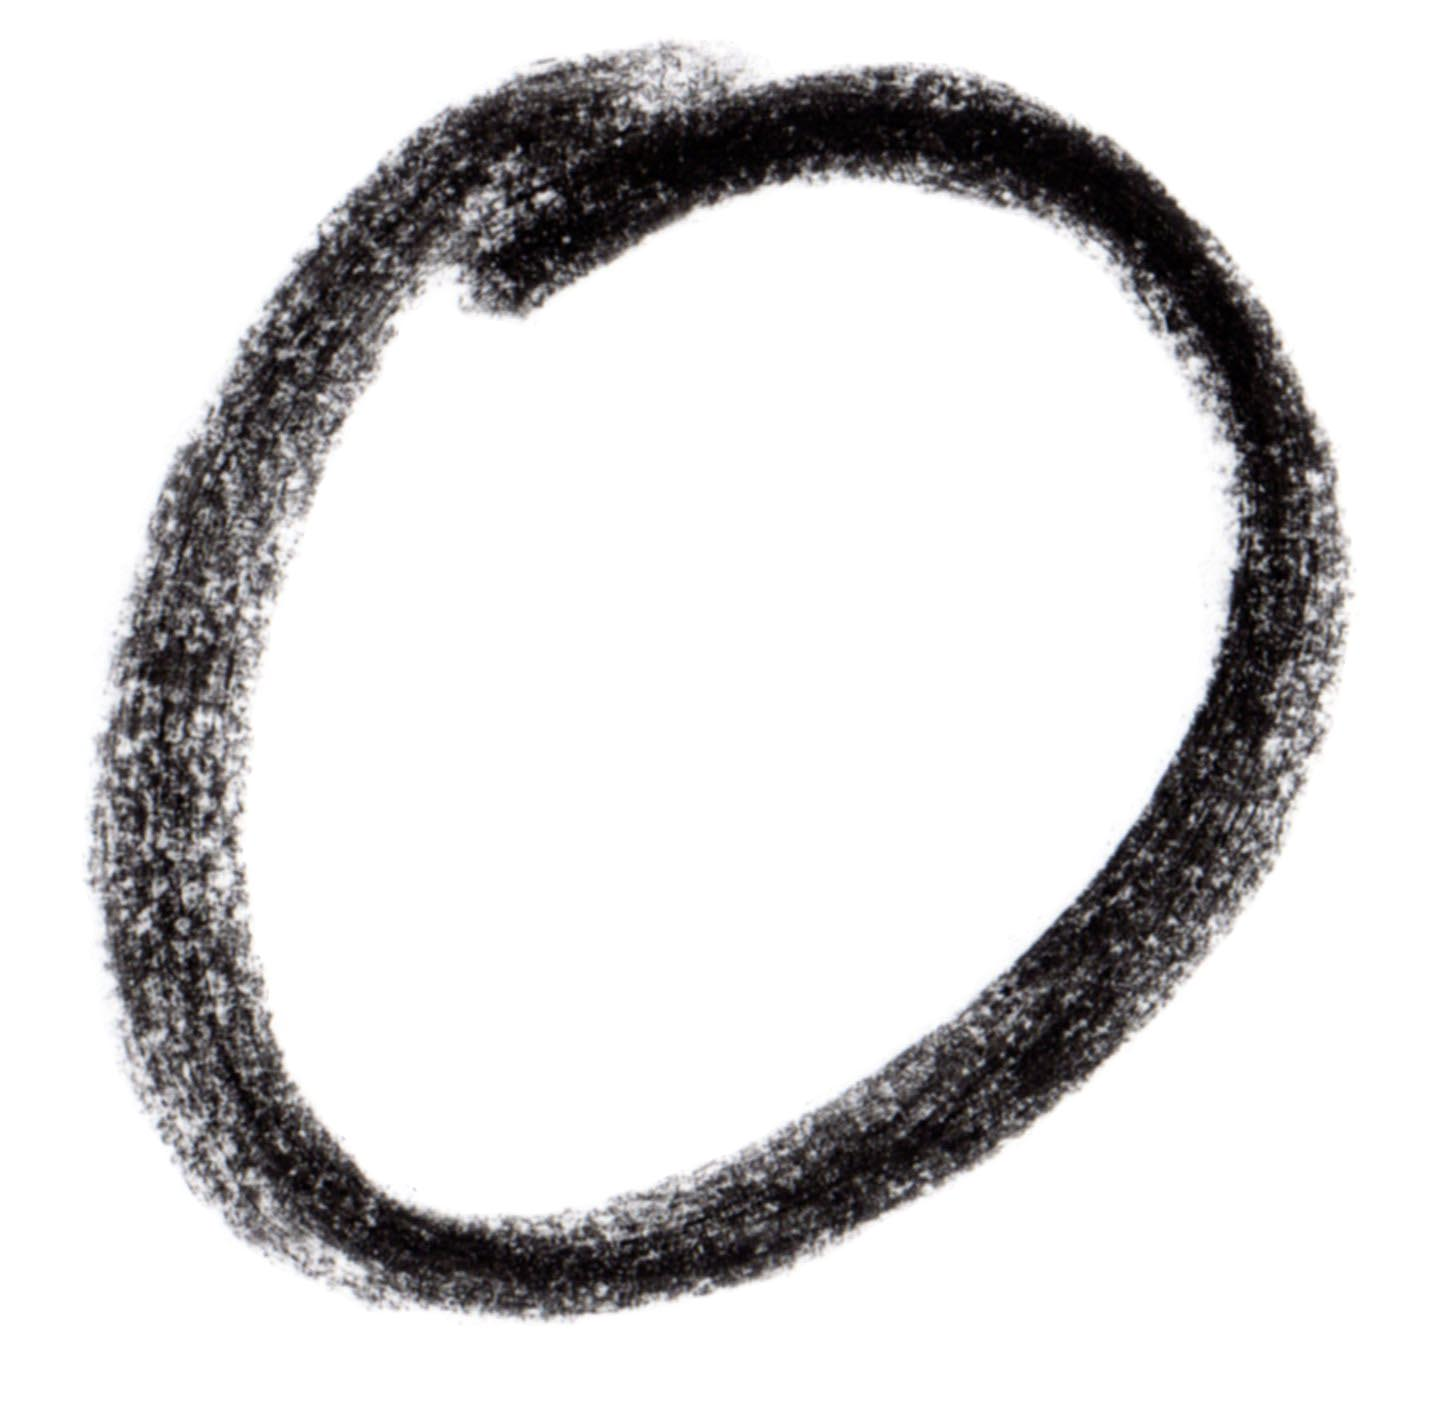
\includegraphics[scale=0.25]{enso.jpg}\\\Enso}
\author{William R. Cook and Tijs van der Storm}
%\date{}                                           % Activate to display a given date or no date

\begin{document}
\maketitle
%\section{}
%\subsection{}


\Enso\ is a theoretically sound and practical reformulation of the 
concepts of model-driven software development. \Enso\ is based
on first-class \textit{structural descriptions}, 
invertable \textit{transformations}, \textit{generic operations} 
and \textit{interpretation}.

Structures in \Enso\ are a specialized kind of graph,
whose nodes are either primitive data or collections of observable
properties, whose values are either nodes or collections of nodes.
From a programming language viewpoint this may seem an odd 
choice for data representation. However, it is essentially the
Entity-Relationship (ER) model \cite{FOO}, also known as Information
Models \cite{FOO}, which is widely used in the design of relational databases
and is also the basis for Class Diagrams in 
the Unified Modeling Language (UML) \cite{FOO}, which 
describe the structure of networks of objects.
The key point is that structures in \Enso\ are 
viewed holistically as \textit{graphs}, not as individual values
or traditional sums-and-products data structures.

A structural description, or \textit{schema}, specifies some 
of the observable properties of structures. Schemas are used to
check the consistency structures. Some properties can be checked
while the structure is being created, but other can only be checked
once the structure is complete. \Enso\ allows modification of structures,
which is necessary to create cyclic graphs, but also allows 
valid structures to be sealed to prevent further changes.

Invertible transformations are used to map one structure into
another kind of structure, such that mapping can be inverted to 
(partially) recover the original structure from the result.
One common kind of transformation is called a \textit{grammar},
which is an invertible transformation between structures and text.
Text grammars are invertable because they can be used for parsing
and also rendering. Other transformations include Diagram grammars,
which map structures into diagrams, were edits on the diagram are
reflected in the original structure. Grammars that describe
the structure and behavior of user interfaces are used to generate
very natural applications.
Transformations are also used for querying, template processing, 
and serialization.

Operations can be guided by schemas or grammars, allowing highly
generic operations to be defined for comparison, differencing, 
merging, projecting and otherwise manipulating cyclic structures.
These operations are cyclic maps, which correspond to coinductive 
transformations.
Since schemas and transformations are also structures, they can
be merged and transformed using these same generic operations.
Transformations on schemas can be applied to instances, to support
upgrade and change management of data.
The resulting system supports powerful modularity constructs,
including feature modules, inheritance, and mixins.

\Enso\ is based on interpretation rather than code generation. 
While it is possible to define transformations that generate code
in conventional languages, this is rarely (if ever) done in \Enso.
Instead all structural descriptions and transformations are 
interpreted dynamically. Although the current incarnation of \Enso\
does not include it, we have previously demonstrated that partial
evaluation can be applied to \Enso-style interpreters to automatically
generate efficient code.

What follows is a rapid introduction to the concepts and use of
\Enso. To avoid too many digressions, 
the many connections between \Enso\ and existing approaches,
including programming models
(model-driven, object-oriented, polytypic, functional, constraint-based), theory (dependent types, coalgebra, category theory),
and related ideas (relational databases, domain-specific languages)
are discussed in Section~\ref{relatedwork}.

\section{Structures}

\subsection{Schemas}

The following schema describes a collection of genealogy information:

\begin{verbatim}
schema GenealogySchema

  class Genealogy
    name: str
    members: Person*

  class Person
    name: str (key)
    birth: date
    female: bool
    father: Person?
    mother: Person?
\end{verbatim}

In a schema, a \textit{class} defines a kind of value, which is
followed by its properties or \textit{fields}. Each field has a name
and a type, where the type may be followed by \C|*| to indicate a 
many-valued field, or by \C|?| to indicate an optional value.
In this case, \C|Genealogy| has \C|members| which is a set of \C|Person|.
A \C|Person| has a \C|name| string, a \C|birth| date, and a \C|father| and \C|mother|,
which are optional \C|Person|s. The \C|father| and \C|mother| are optional
because every geneology is partial, so that not all fathers and mothers
can be included.

\subsection{Data}

A particular collection of genealogy information, which conforms to the
above schema, might be written as follows:

\begin{verbatim}
Genealogy "Sam's Ancestors"
Person "Albert Snook"  11/1/89 male  +"Jane Snook" ^"Thomas Snook"
Person "Jane Snook"    3/17/48 female 
Person "Thomas Snook" 12/30/43 male 
\end{verbatim}

\subsection{Inverses}

\subsection{Factories}

Structure are created by \textit{factories}, which create
and manage the nodes in the structure. The factory also
ensures that structures are distinct: a factory identifies the 
collection of nodes that belong to a graph, and any given node 
can only be connected to other nodes in the same graph, which were
created by the same factory.

In \Enso\ most properties of a structure are
checked when the structure is being created. In other words, 
the \textit{factory} that creates the structure is parameterized by a
schema, which the factory uses to check the legality of operations
on the objects it creates.

\section{Grammars}

\subsection{Textual Grammars}


\subsection{Instantiation}





\subsection{Relationship to Other Approaches}
\label{relatedwork}

\Enso\ data is based on traditional 
entity-relationship (ER) models \cite{FOO},
which are also known as information models. 
ER models were the basis for class diagrams in UML.

In contrast to
object-oriented programming, \Enso\ is focused on holistic
object graphs, rather than individual objects. \Enso\ 
does allow data to include some behavior, for example constraints
and computed fields, but \Enso\ does not associated methods
with data objects.

In contrast to
most theories of functional programming, \Enso\ is based on
coalgebraic signatures rather than algebraic ones. In practice
this means that \Enso\ structures are cyclic graphs rather than
trees. Lazy functional languages can also represent cyclic 
structures, but the cycles are not observable.

\Enso\ supports controlled imperative effects. Objects are
mutable during construction or modification, while the data may be in an
inconstent state, but before it can be used it must be validated
and locked from further changes. This is similar to a transaction.


The rendering transformation is similar to Smaragdakis's notion of
Morphing \cite{Morphing} (or is it SafeGen?). 
However, \Enso\ generalizes the transformation
so that any kind of structure can be morphed into any other
kind of structure. On the other hand, \Enso\ is not statically
typed.

\Enso's generic operations are a form of polytypic programming, 
like Generic Haskell \cite{TH}. \Enso's operations can use
arbitrary meta-data, not just sum/product type structure.
On the other hand, \Enso's operations are not statically typed.
\Enso\ certainly shares the same goal to ``Write everything once''.

\subsection{Other Related Work}

Look up work on "instant-generics"


Eelco Lempsink, Sean Leather, and Andres L\&\#246;h. 2009. Type-safe diff for families of datatypes. In Proceedings of the 2009 ACM SIGPLAN workshop on Generic programming (WGP '09). ACM, New York, NY, USA, 61-72. DOI=10.1145/1596614.1596624 http://doi.acm.org/10.1145/1596614.1596624 

Dave Clarke, Michiel Helvensteijn, and Ina Schaefer. 2010. Abstract delta modeling. In Proceedings of the ninth international conference on Generative programming and component engineering (GPCE '10). ACM, New York, NY, USA, 13-22. DOI=10.1145/1868294.1868298 http://doi.acm.org/10.1145/1868294.1868298 

Data Representation Synthesis
Peter Hawkins, Alex Aiken, Kathleen Fisher, Martin Rinard, Mooly Sagiv. In Programming Language Design and Implementation (PLDI), ACM, 2011

\subsection{FOSD}


- Forests are the key data structure in a formal model of FOSD [1]. The goal is similar to yours: be language-independent and represent object collaborations.

- Recently, forests have been extended to graphs to encode more semantics and to support more automatic reasoning activities [2].

- Operations on forests (e.g., composition or conflict detection) are defined generically and can be plugged in on demand [3].

- The entire FOSD model is language-independent and has been used with many different artifact types (e.g., Java, C, Haskell, Alloy programs) [3].

- FOSD tools (the internal parsers and reasoning tools) are generated based on annotated grammars, whose annotations supply semantic information [3].

- The entire forest/grammar/annotation-based model has been enriched by adding behavior to features [4]. 

[1] Sven Apel, Christian Lengauer, Bernhard M�ller, and Christian K�stner. An Algebraic Foundation for Automatic Feature-Based Program Synthesis. Science of Computer Programming (SCP), 75(11):1022�1047, November 2010.

[2] Sven Apel, Wolfgang Scholz, Christian Lengauer, and Christian K�stner. Language-Independent Reference Checking in Software Product Lines. In Proceedings of the International Workshop on Feature-Oriented Software Development (FOSD), pages 65�71. ACM Press, October 2010.

[3] Sven Apel, Christian K�stner, and Christian Lengauer. FeatureHouse: Language-Independent, Automated Software Composition. In Proceedings of the ACM/IEEE International Conference on Software Engineering (ICSE), pages 221�231. IEEE Computer Society, May 2009.

[4] P. H�fner, R. Khedri, B. M�ller. Supplementing Product Families with Behaviour. International Journal of Software and Informatics, 2011. To appear. 

Dave Clarke, Michiel Helvensteijn, Ina Schaefer. Abstract delta modeling. GPCE'10

\section{Notes}

Grammar equivalence should ignore differences of non-terminals.
That is, inserting a new definition is not an "equal" grammar,
but it can be "equivalent" observably. For example

\begin{verbatim}
A = "one" "two"

B = "one" C
C = "two"
\end{verbatim}

We should say that A and B are equivalent. To make this
work, equivalence has to be able to reason about "stutter"
steps in the state machines. This is similar to the
fact that Alt is injective in the grammar schema, and
the injection is sometimes needed during rendering.
By injective I mean that Alt([A])==A, or that an Alt with
one sub-time is the same as the subitem itself. 
Sequence is also injective, Seq([A])==A. These differences
should be ignored by equivalence. If we put a boolean on 
klasses in the schema schema for "injective" then this could
be implemented. 

We should also implement unordered collections. 
I wonder how hard this would be to add in a feature-oriented way.
Every time we add a feature we should refactor the interpreter
code to make it possible. Eventually we will have very
extensible interpreters.

\section{Requirements for a programming language}

The programming model is based on cyclic graphs.
Graphs are kept distinct from each other. That is,
each graph is considered a self-contained
artifact, without links or pointers to other graphs.

A natural way to create such graphs is with 
imperative effects.

This potentially requires more copying of data
than would be the case in tree-based representations.

To modify graphs, place-holder objects are useful,
as is the ability to "become" another object.

\subsection{Simple reflection}

Fields can be created dynamically and accessed with
"." notation or reflective access.

\begin{verbatim}
o.foo   == o.get("foo")
\end{verbatim}

Assignment to fields can be overriden
\begin{verbatim}
   o.bar = 3   ==> o.set("bar", 3)
\end{verbatim}



\section{QuadModel}


\begin{figure}[htbp]
\begin{center}
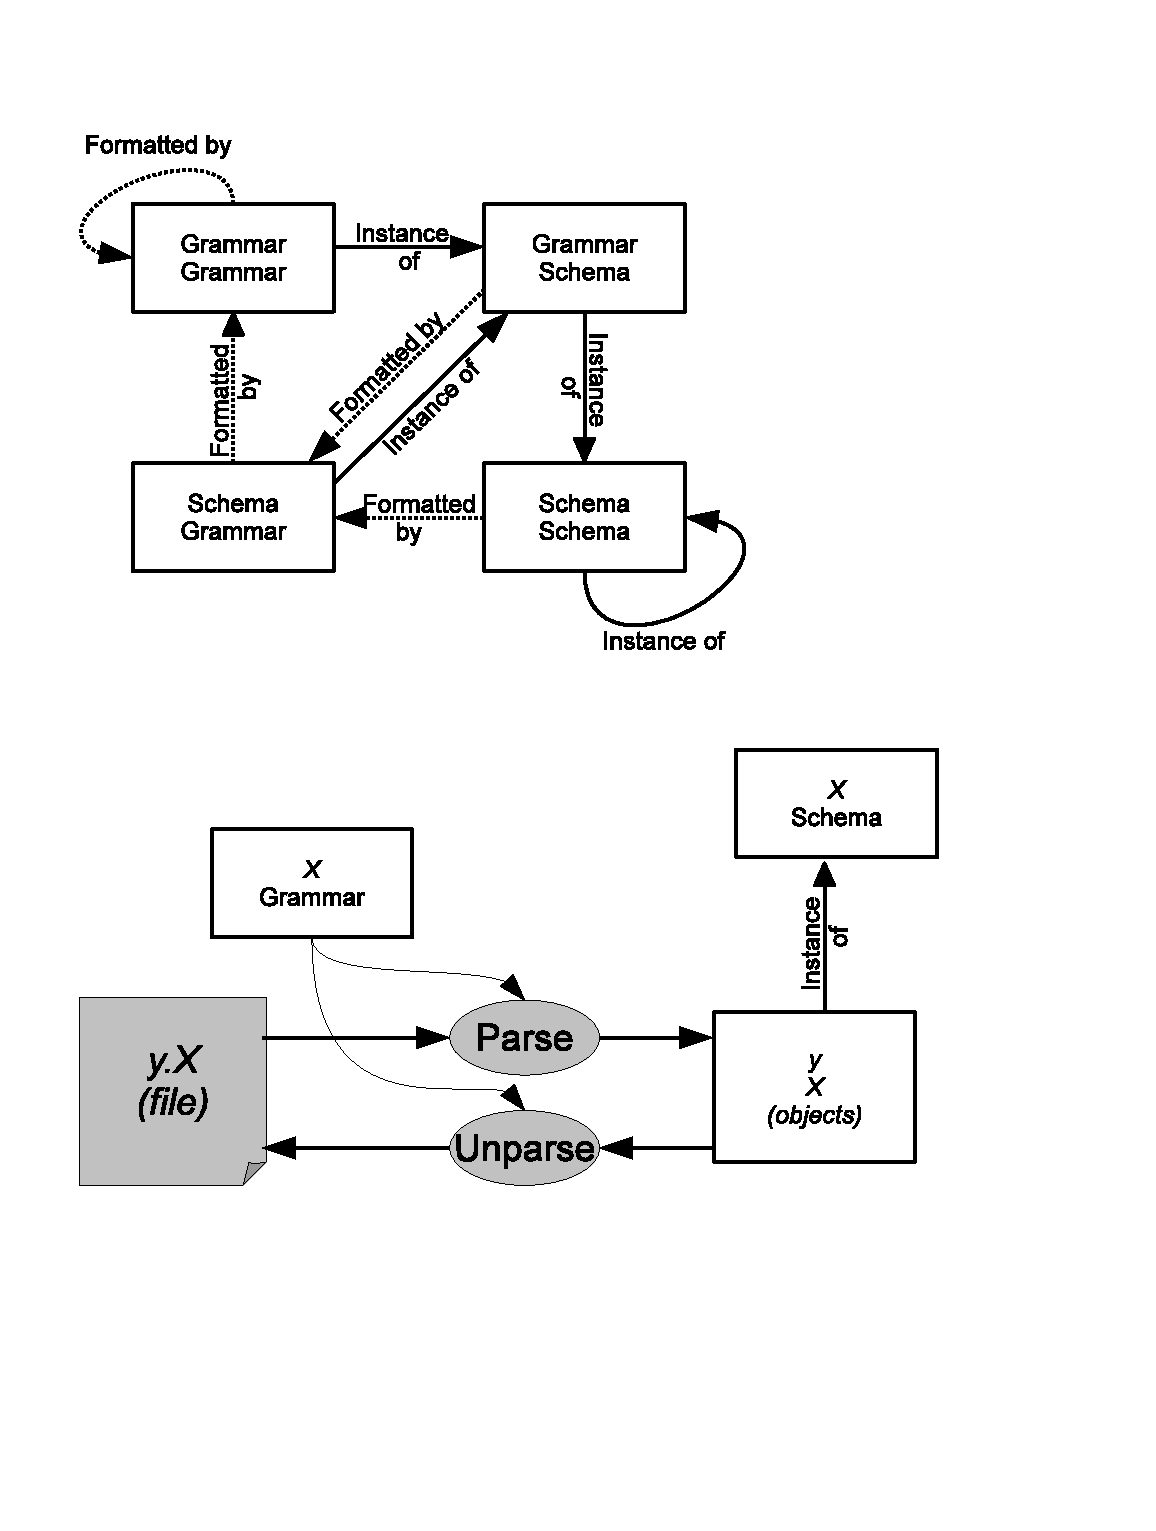
\includegraphics[scale=0.7]{QuadModel.pdf}
\caption{The four core schema and grammar models}
\label{default}
\end{center}
\end{figure}

\begin{figure}[htbp]
\begin{center}
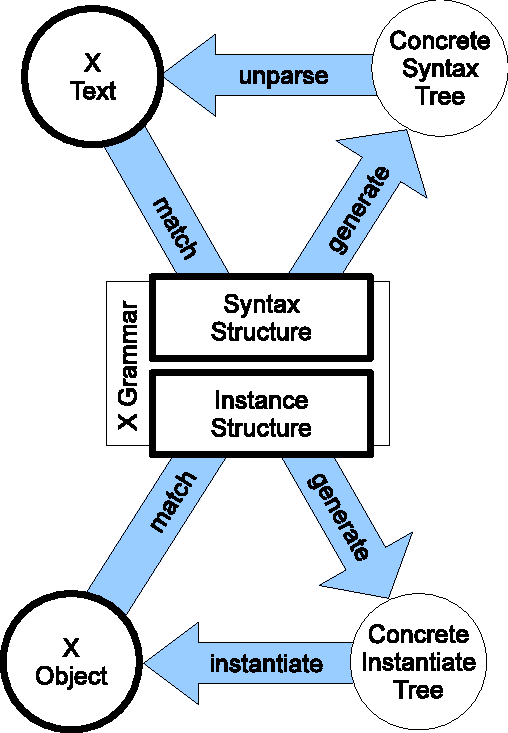
\includegraphics[scale=0.7]{ParseRender1.pdf}
\caption{Invertable grammar transformations}
\label{default}
\end{center}
\end{figure}
\begin{figure}[htbp]
\begin{center}
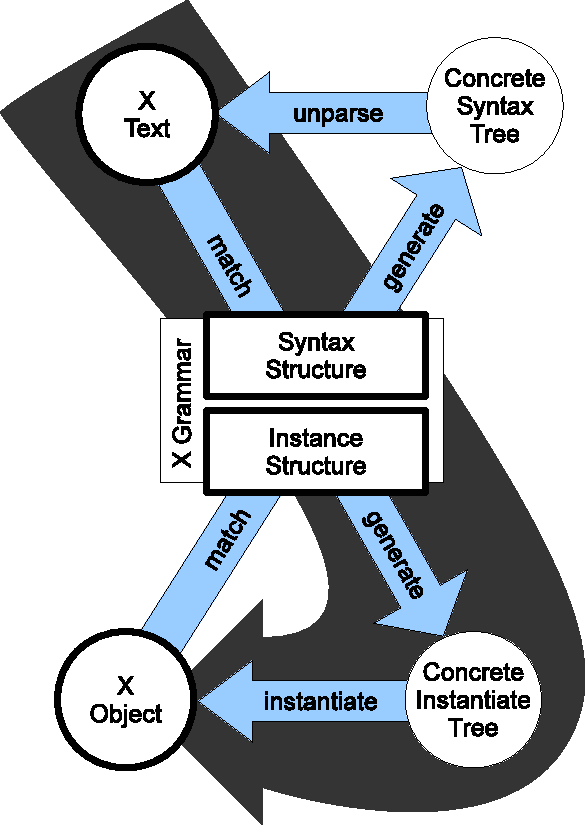
\includegraphics[scale=0.7]{ParseRender2.pdf}
\caption{Parsing matches \textit{syntactic structure} and generates \textit{instance structure}}
\label{default}
\end{center}
\end{figure}
\begin{figure}[htbp]
\begin{center}
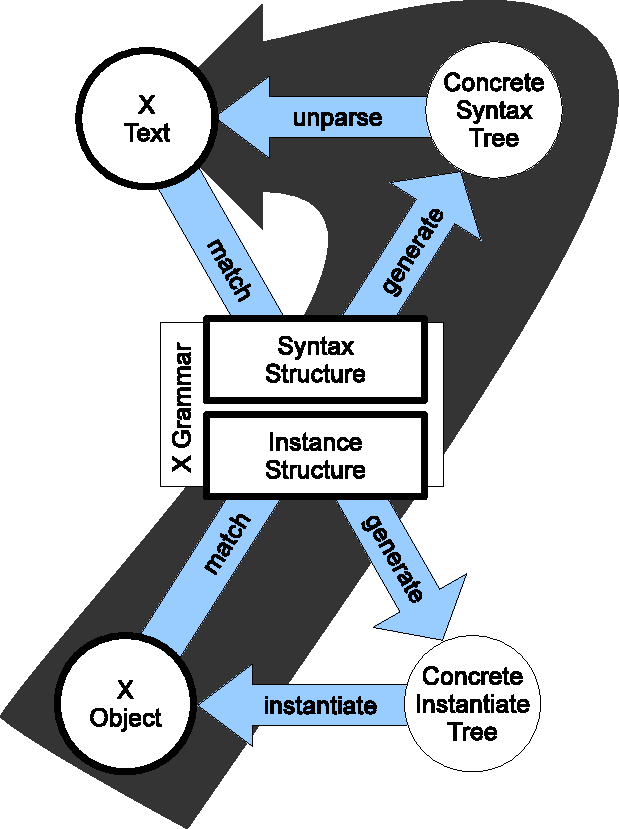
\includegraphics[scale=0.7]{ParseRender3.pdf}
\caption{Rendering matches \textit{instance structure} and generates \textit{syntactic structure}}
\label{default}
\end{center}
\end{figure}
\begin{figure}[htbp]
\begin{center}
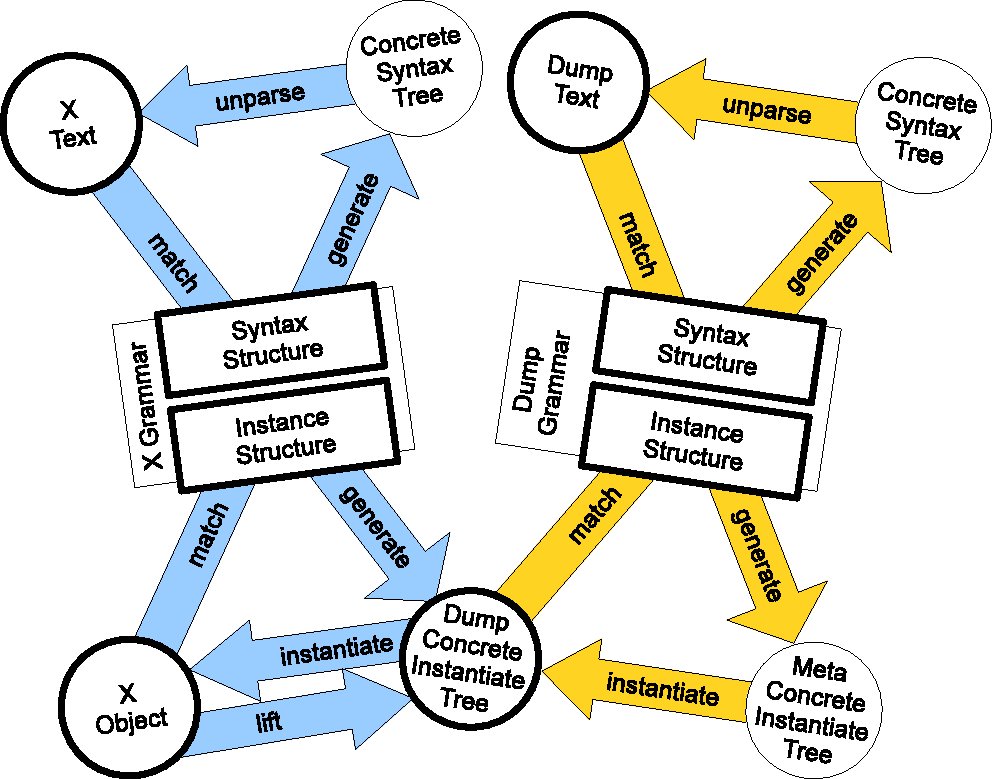
\includegraphics[scale=0.7]{ParseRender4.pdf}
\caption{Relationship between parsing and dumping}
\label{default}
\end{center}
\end{figure}
\begin{figure}[htbp]
\begin{center}
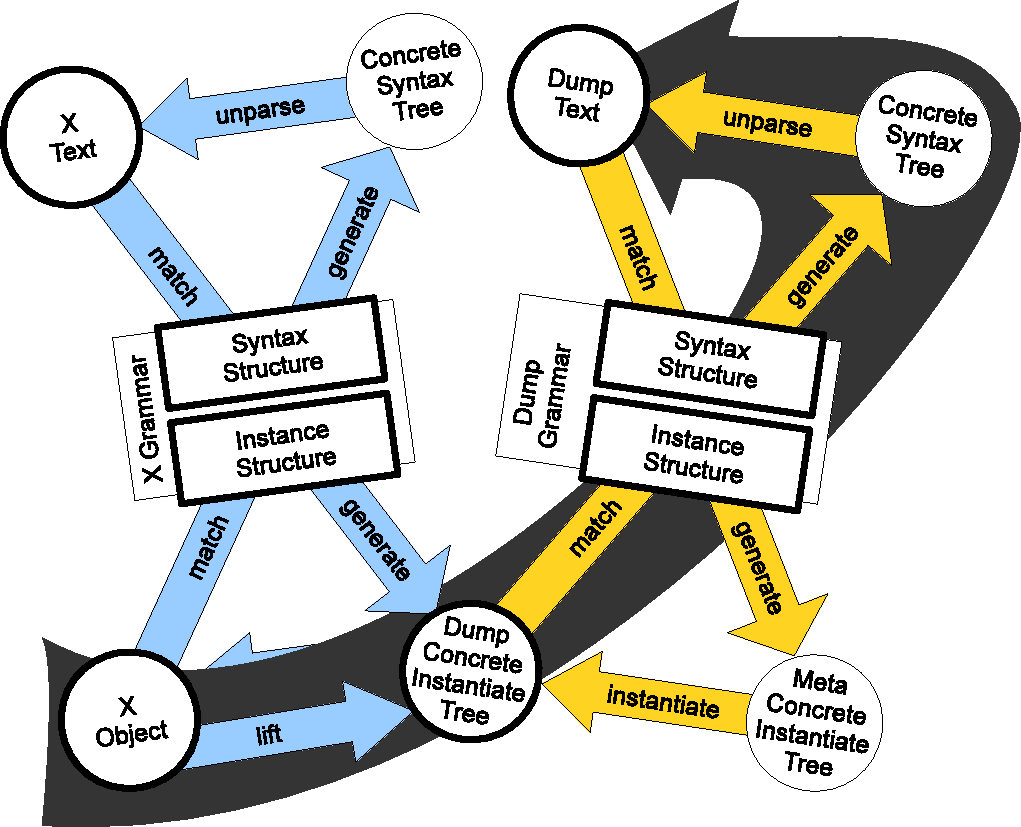
\includegraphics[scale=0.7]{ParseRender5.pdf}
\caption{Rendering to dump format}
\label{default}
\end{center}
\end{figure}

\begin{figure}[htbp]
\begin{center}
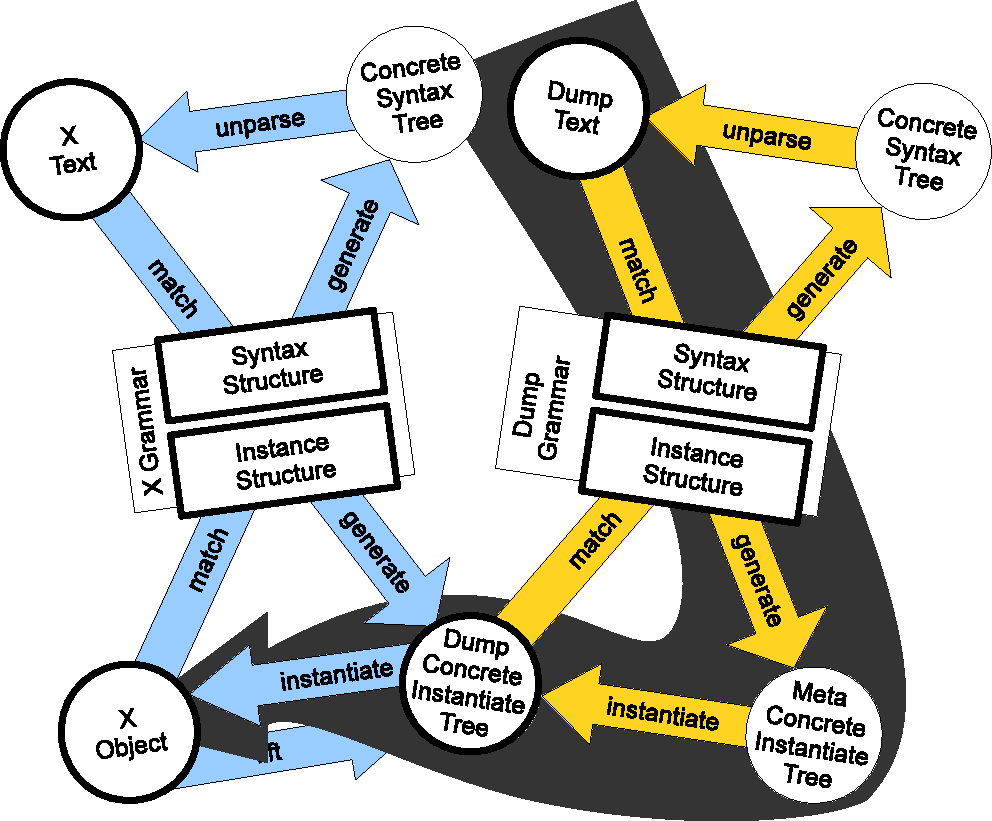
\includegraphics[scale=0.7]{ParseRender6.pdf}
\caption{Reading dump format to create objects}
\label{default}
\end{center}
\end{figure}


\end{document}  



\begin{verbatim}
schema Geometry

class Shape

class Point < Shape
  x: int
  y: int

class Rectangle < Shape
  upper_left: Point
  lower_right: Point

class Circle < Shape
  center: Point
  radius: int

class Polygon < Shape
  points: Point*
  
class Composite < Shape
  items: Shape*
\end{verbatim}

It says that the class \C|Point| has fields \C|x| and \C|y|.
--------
This example converts schemas into constructor grammars
\begin{verbatim}
grammar NAME:sym
   CLASSES:
     rule NAME:sym = 
        (SUBTYPES: { NAME:sym "|") "|" @"!SUBTYPES.empty?")?
         [NAME:sym] NAME:str "{" 
            FIELDS: { (NAME:str ":" (NAME:sym): (
                 "[" { TYPE.NAME:sym^ "," } "]"   @"MANY=true"
               | TYPE.NAME:sym^ ?                  @"OPTIONAL=true"
               | TYPE.NAME:sym^
               )) ";" }
             "}"
\end{verbatim}


<%
Contributions of this work:
- 

How we do it:
- s

%>




\input{conclusion}


%
% The following two commands are all you need in the
% initial runs of your .tex file to
% produce the bibliography for the citations in your paper.
\bibliographystyle{abbrv}
\bibliography{interpreter}  % sigproc.bib is the name of the Bibliography in this case
% You must have a proper ".bib" file
%  and remember to run:
% latex bibtex latex latex
% to resolve all references
%
% ACM needs 'a single self-contained file'!
%

\end{document}

